\documentclass{beamer}
%\documentclass{article}
%\usepackage{beamerarticle}

\newlength{\px}
\setlength{\px}{0.0009765625\paperwidth}

\usetheme[footline=authortitle,compress]{Nomeata}
%\usecolortheme{orchid}
\usecolortheme{crane}

\usepackage[german]{babel}
\usepackage[utf8]{inputenc}
\usepackage{tikz}
%\usetikzlibrary{shapes,arrows}
\usetikzlibrary{positioning,calc,decorations,decorations.pathmorphing,shapes.symbols}
\usepackage{hyperref}

\usepackage{listings}

% \pause mit verstecken
\newcommand{\hide}{\onslide+<+(1)->}

\title{Freie Werkzeuge für die technische Dokumentation}
\subtitle{}
\author{Joachim Breitner}
%\institute{\url{mail@joachim-breitner.de}}
%\titlegraphic{
\includegraphics[width=100pt]{itomig-logo}}
\date{tfk Technologietag in München\\9. März 2010}

\begin{document}

\frame[plain]{\titlepage}
\only<article>{\maketitle}

\section{Die Problemstellung}
\only<presentation>{\subsection*{}}

\begin{frame}
\frametitle{Die Crux mit den Word-Dateien}
\begin{center}
\begin{tikzpicture}

\visible<3->{
\node (typ1) at (-3,0) {
\includegraphics[width=12mm]{typ1}};

\node (typ2) at (3,0) {
\includegraphics[width=12mm]{typ2}};
}

\visible<3,7->{
\draw[->,color=blue,line width=1.5mm] ($(typ1.east) + (0,.2)$)  -- ($(typ2.west)+(0,.2)$);
}

\visible<4,7->{
\draw[->,color=blue,line width=1.5mm] ($(typ2.west) - (0,.2)$) --  node[below] (word) {
\includegraphics[width=10mm]{word}} ($(typ1.east)-(0,.2)$);
}

\visible<-3,7->{
\path ($(typ1.east) + (0,.2)$) -- node[above] (word) {
\includegraphics[width=10mm]{word}} ($(typ2.west)+(0,.2)$);
}

\visible<5-6>{
\node at ($(typ1.west)+(-.3,-.3)$) {
\includegraphics[width=10mm]{word}};
}
\visible<6>{
\node at ($(typ2.east)+(.3,-.3)$) {
\includegraphics[width=10mm]{word}};
}

\visible<8>{
\node (typ3) at (-3,-3) {
\includegraphics[width=12mm]{typ3}};

\node (typ4) at (3,-3) {
\includegraphics[width=12mm]{typ4}};

\draw[->,color=blue,line width=1.5mm,shorten <=3mm] (typ1) --  node[left]  {
\includegraphics[width=10mm]{word}} (typ4);
\draw[->,color=blue,line width=1.5mm] (typ1) --  node[left]  {
\includegraphics[width=10mm]{word}} (typ3);
\draw[->,color=blue,line width=1.5mm] (typ3) --  node[below]  {
\includegraphics[width=10mm]{word}} (typ4);
\draw[->,color=blue,line width=1.5mm] (typ4) --  node[right]  {
\includegraphics[width=10mm]{word}} (typ2);

}

\visible<2>{
\node[text width=4cm,fill=white] at ($(word) + (3,-4)$) (txt) {
Dieser \textbf{Text} ist alles {\color{red}andere \emph{als}} {\Large einheitlich}, und \underline{jeder} \textsc{Autor} wurschtelt herum \textrm{wie} \textrm{er} will!
};
\draw[rounded corners] ($(txt.south west)+(0,-.5em)$) -- (txt.north west) -- (txt.north east) -- ($(txt.south east)+(0,-.5em)$);
\draw[decorate,decoration={zigzag,raise=-.4em}] ($(txt.south east)+(0,-.5em)$) -- ($(txt.south west)+(0,-.5em)$);
\draw[->,color=yellow,line width=1.5mm,shorten <=2mm] (txt) -- (word);
}
\end{tikzpicture}
\end{center}
\end{frame}

\begin{frame}
\frametitle{Die Crux mit den Word-Dateien}
\begin{enumerate}
\item Kein einheitliches Layout 
\item Konflikte bei zeitgleicher Beareitung 
\item Änderungen sind schwer nachzuvollziehen und zuzuordnen 
\end{enumerate}
\end{frame}


\section{Freie Software}
\only<presentation>{\subsection*{}}

\begin{frame}
\frametitle{Was ist Freie Software?}

Der Kunde hat bei das Recht, die Software
\begin{enumerate}
\item frei zu verwenden.
\item frei zu studieren.
\item frei zu verändern.
\item frei weiterzugeben.
\end{enumerate}

\begin{block}{Bekannte Freie Software}
\begin{center}
\hfill

\includegraphics[height=120\px]{firefox}
\hfill

\includegraphics[height=120\px]{openoffice}
\hfill

\includegraphics[height=120\px]{tux}
\hfill
\strut
\end{center}
\end{block}

\end{frame}

\begin{frame}
\frametitle{Was bedeutet Freie Software im Firmeneinsatz?}
\begin{itemize}
\item Keine Lizenzkosten
\item Keine restriktiven Lizenzbedingungen
\item Überprüfbare Sicherheit
\item Unbeschränkt anpassbar
\item Unabhängigkeit von einem Hersteller
\item Investitionssicherheit
\end{itemize}
\end{frame}

\begin{frame}
\frametitle{Wie kann man damit Geld verdienen?}
\begin{itemize}
\item Erstentwicklung
\item Support
\item Auftragsentwicklung
\item ggf. Hosting
\end{itemize}
\end{frame}

\section{DocBook}
\only<presentation>{\subsection*{}}

\begin{frame}[fragile]
\lstset{language=XML,basicstyle=\small\ttfamily}
\frametitle{Lösung 1: DocBook}

\lstinputlisting{simple.xml}
\end{frame}

\begin{frame}
\frametitle{Was ist DocBook}
\begin{itemize}
\item Beschreibungssprache für Dokumente, ähnlich HTML
\item Ein XML-Dialekt
\item Ausgelegt für technische Dokumente (Hardware und Software)
\item Strenge Trennung von Inhalt und Layout
\item Ausgabe als PDF, HTML, CHM, etc. möglich
\item Layout wird über \emph{Stylesheets} definiert
\end{itemize}
\end{frame}

\begin{frame}
\frametitle{Allergie gegen XML-Syntax?}
\begin{center}
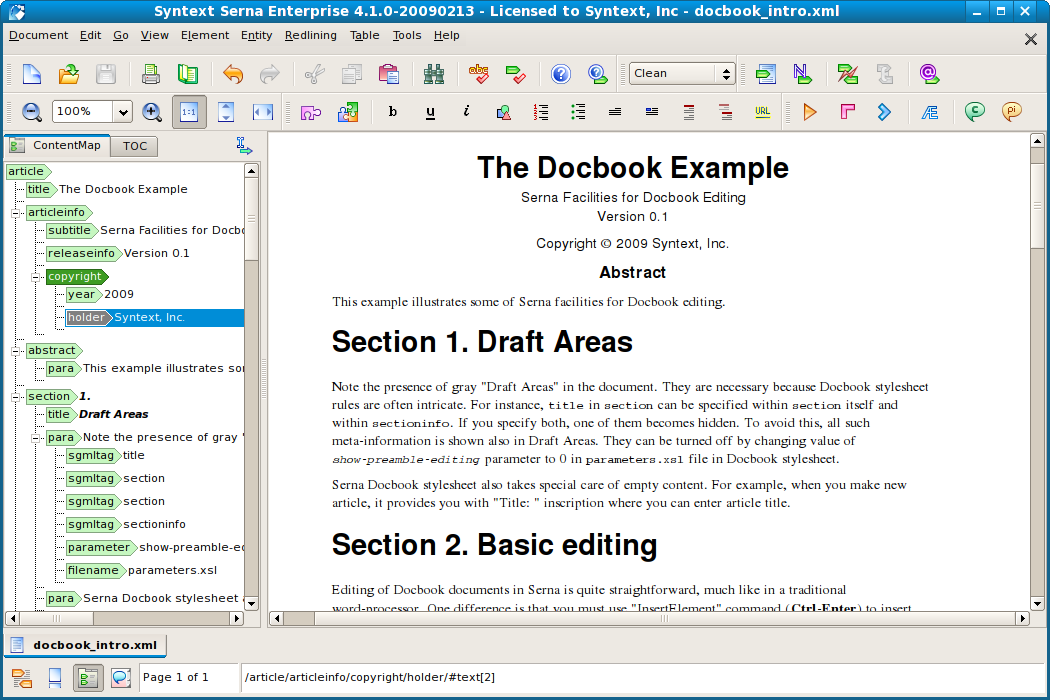
\includegraphics[width=\linewidth]{serna-screenshot}
\end{center}
\end{frame}

\begin{frame}
\frametitle{Allergie gegen XML-Syntax?}
Es gibt auch graphische XML-Editoren mit spezieller DocBook-Unterstützung
\begin{enumerate}
\item Serna XML Editor \emph{(auch als OpenSource-Produkt erhältlich)}
\item XMLmind Editor
\item Oxygen XML Editor
\end{enumerate}
\end{frame}


\section{Subversion}
\only<presentation>{\subsection*{}}

\begin{frame}
\frametitle{Lösung 2: Subversion}
\begin{center}
\begin{tikzpicture}

\visible<1-2>{
\node (typ1) at (-3,0) {
\includegraphics[width=12mm]{typ1}};

\node (typ2) at (3,0) {
\includegraphics[width=12mm]{typ2}};

\draw[->,color=blue,line width=1.5mm] ($(typ1.east) + (0,.2)$)  -- ($(typ2.west)+(0,.2)$);

\draw[->,color=blue,line width=1.5mm] ($(typ2.west) - (0,.2)$) --  node[below] (word) {
\includegraphics[width=10mm]{word}} ($(typ1.east)-(0,.2)$);

\path ($(typ1.east) + (0,.2)$) -- node[above] (word) {
\includegraphics[width=10mm]{word}} ($(typ2.west)+(0,.2)$);

\node (typ3) at (-3,-3) {
\includegraphics[width=12mm]{typ3}};

\node (typ4) at (3,-3) {
\includegraphics[width=12mm]{typ4}};

\draw[->,color=blue,line width=1.5mm,shorten <=3mm] (typ1) --  node[left]  {
\includegraphics[width=10mm]{word}} (typ4);
\draw[->,color=blue,line width=1.5mm] (typ1) --  node[left]  {
\includegraphics[width=10mm]{word}} (typ3);
\draw[->,color=blue,line width=1.5mm] (typ3) --  node[below]  {
\includegraphics[width=10mm]{word}} (typ4);
\draw[->,color=blue,line width=1.5mm] (typ4) --  node[right]  {
\includegraphics[width=10mm]{word}} (typ2);
}
\visible<2>{
\node[forbidden sign,minimum size=4cm,draw=red,line width=5mm] at ($1/2*(typ1) + 1/2*(typ4)$) {};
}
\end{tikzpicture}
\end{center}
\end{frame}

\begin{frame}
\frametitle{Lösung 2: Subversion}
\begin{center}
\begin{tikzpicture}
\node (server) {\includegraphics[width=18mm]{server}};
\visible<2->{

\node (typ1) at (-3,-5) {
\includegraphics[width=12mm]{typ1}};
\node (typ2) at (-1,-5) {
\includegraphics[width=12mm]{typ2}};
\node (typ3) at (1,-5) {
\includegraphics[width=12mm]{typ3}};
\node (typ4) at (3,-5) {
\includegraphics[width=12mm]{typ4}};

\draw[<->,color=blue,line width=1.5mm] (typ1) --  node[left]  {
\includegraphics[width=10mm]{word}} (server);
\draw[<->,color=blue,line width=1.5mm] (typ2) --  node[left]  {
\includegraphics[width=10mm]{word}} (server);
\draw[<->,color=blue,line width=1.5mm] (typ3) --  node[right]  {
\includegraphics[width=10mm]{word}} (server);
\draw[<->,color=blue,line width=1.5mm] (typ4) --  node[right]  {
\includegraphics[width=10mm]{word}} (server);
}
\end{tikzpicture}
\end{center}
\end{frame}

\begin{frame}
\frametitle{Was ist Subversion}
\begin{itemize}
\item Freie Software zur versionierten Dateiverwaltung
\item Daten und deren Historie werden zentral vorgehalten.
\item Anwender arbeiten im lokalen Repository.
\item Änderungen werden kommentiert.
\item Konflikte werden erkannt und, falls möglich, automatisch aufgelöst.
\item Authentifizierung über den Webserver Apache (und damit LDAP, Active Directory etc.) möglich
% \item Versionsstände können mit \emph{Tags} markiert werden.
\item Es existieren Clients für Windows, die sich in den Windows Exporer integrieren.
\end{itemize}
\end{frame}

% \begin{frame}
% \frametitle{Ein Typischer Subversion-Ablauf}
% \begin{enumerate}
% \item Der Benutzer zieht eine Arbeitskopie der Dateien auf seinen Rechner (\emph{Checkout}).
% \item Er arbeitet lokal wie gewohnt.
% \item Nach jedem geeigneten Arbeitsschritt läd er seine Änderungen mit Kommentar hoch (\emph{Commit}).
% \item Die Kollegin aktualisiert ihre Arbeitsversion auf den neusten Stand (\emph{Update})
% \end{enumerate}
% \end{frame}


\section{zpub}
\only<presentation>{\subsection*{}}

\begin{frame}
\frametitle{Die Kombination: zpub}
\begin{center}
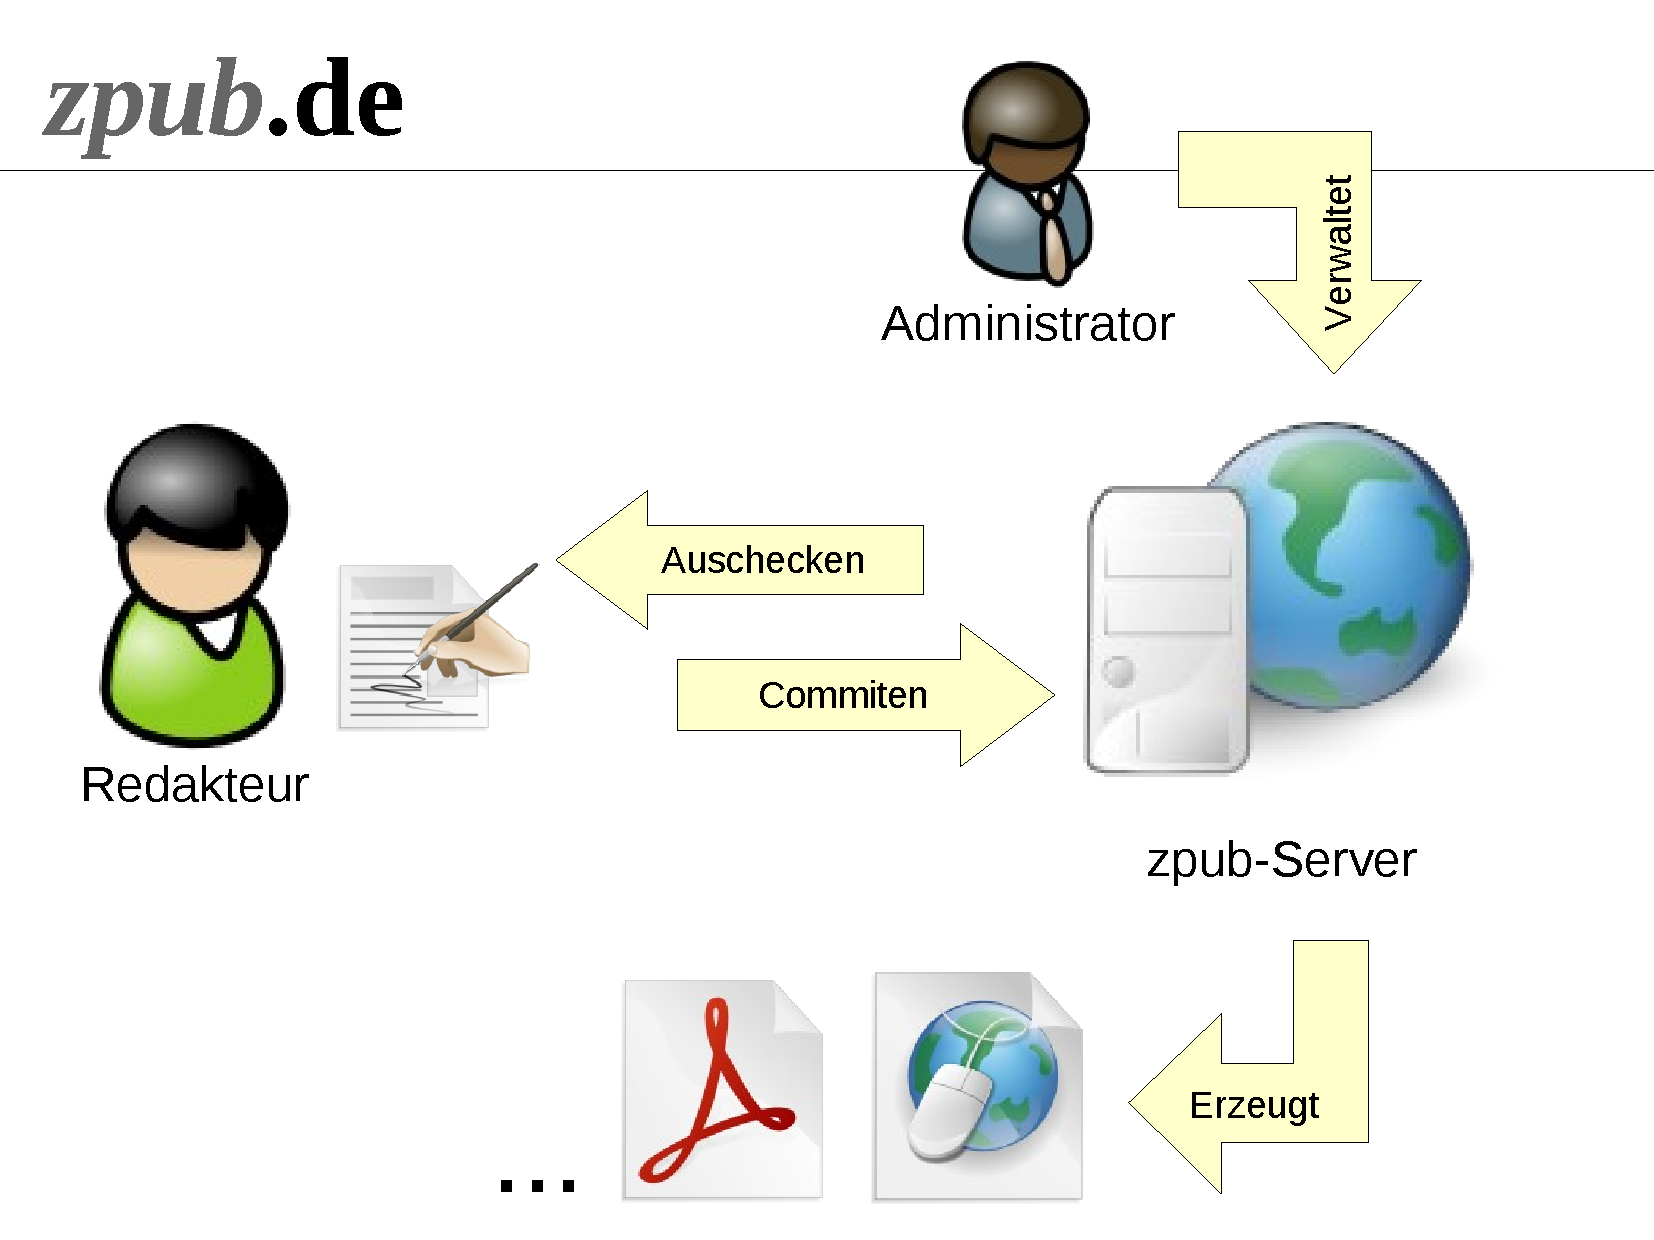
\includegraphics[height=.8\textheight]{zpub-struktur}
\end{center}
\end{frame}


\begin{frame}
\frametitle{Die zpub-Weboberfläche}
\begin{center}
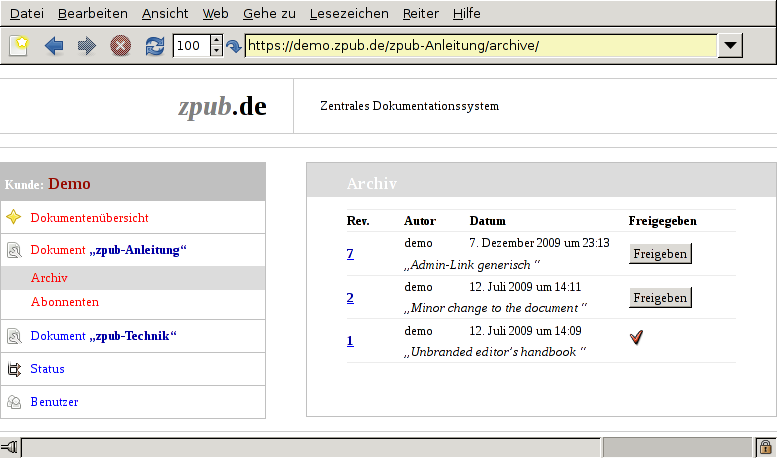
\includegraphics[width=.75878906\paperwidth]{zpub-screenshot}
\end{center}
\end{frame}

\begin{frame}
\frametitle{zpub: Zentrales Dokumentationssystem}
\begin{itemize}
\item Freie Software
\item Integriert DocBook und Subversion
\item Keine DocBook-Tools auf dem Client nötig
\item Ausgabeformate: PDF, HTML, CHM, RTF
\item Platformunabhängig:\\ Anwender verwenden SVN-Client und XML-Editor ihrer Wahl
\item Vollständiges Archiv der früheren Versionen
\item Einfaches Workflow-Management
\end{itemize}
\end{frame}


\section{Fazit}
\only<presentation>{\subsection*{}}

\begin{frame}
\frametitle{Fazit}
\begin{block}{ 100\% Freie Software: }
\begin{itemize}
\item DocBook
\begin{itemize}
\item für überzeugende Dokumente
\item \url{http://www.docbook.org/}
\end{itemize}
\item Subversion
\begin{itemize}
\item für reibungslose Zusammenarbeit an den Dokumenten
\item \url{http://svnbook.red-bean.com/}
\end{itemize}
\item zpub
\begin{itemize}
\item für die komfortable Integration
\item \url{http://zpub.de/}
\end{itemize}
\end{itemize}
\end{block}
\end{frame}


\only<presentation>{\section{}\subsection*{}}

\setbeamercolor{normal text}{bg=black}
\setbeamertemplate{background canvas}{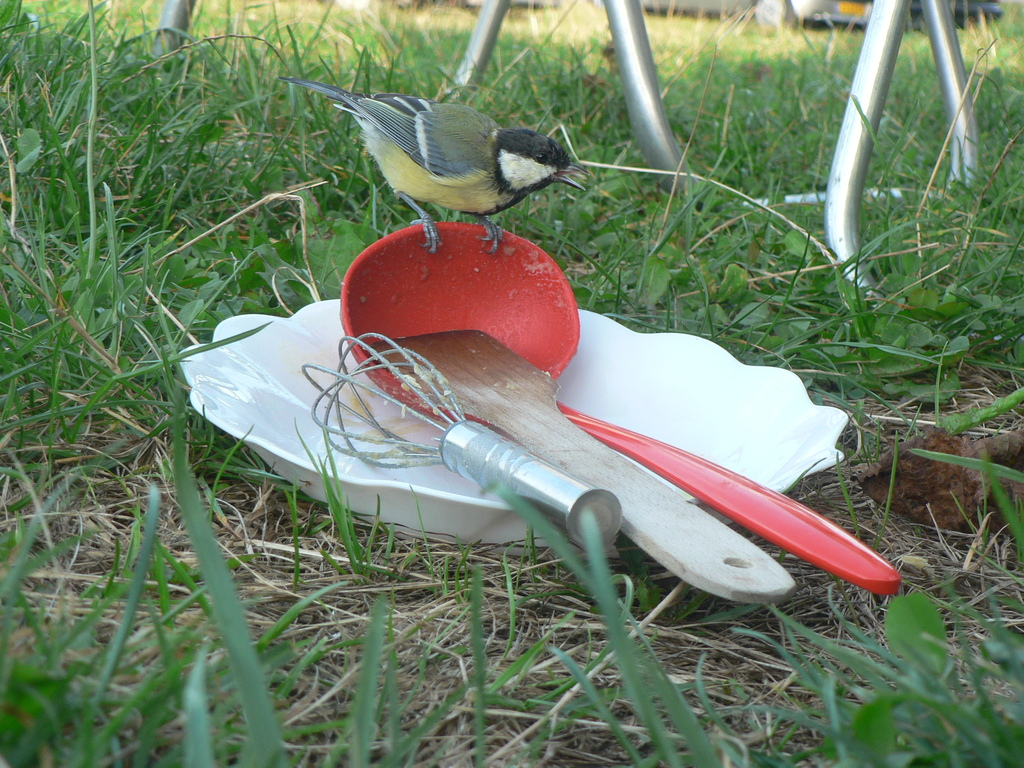
\includegraphics[height=\paperheight,width=\paperwidth]{endbild}}
\frame<presentation>[plain]{}
\end{document}

